\section{Experimental Evaluation}
\label{sec:results}

We evaluate \Treebeard{} on four different target processors, a low resource NVIDIA T400 GPU with 2GB RAM, a medium-tier NVIDIA RTX 4060 GPU with 8GB RAM, a large AMD MI210 GPU with 64GB RAM, and an 
Intel Core i9 CPU  with 16 virtual cores and 128 GB RAM. We compare \Treebeard{} with 
four other systems, NVIDIA RAPIDS\cite{RAPIDS} v23.10, Tahoe\cite{Tahoe}, XGBoost\cite{XGBoost}
v1.7.6 and \TreebeardOLD{}\cite{Treebeard} CPU. 
We measure both kernel time and total time (including data transfer to the GPU and results back) 
for all GPU systems except Tahoe. Tahoe only allows us to measure the kernel time since it is written
as an executable that performs inference repeatedly on the same data that is transferred to the GPU once.
For \Treebeard{}, we use schedules found using the schedule exploration
heuristic (Section \ref{sec:exploring}) unless otherwise specified.

We use two sets of benchmarks to perform the comparison.
We use 8 real-world models trained on data from the Intel Machine 
Learning Benchmark suite~\cite{MLBenchmarks}. These models were also
used to evaluate \TreebeardOLD{}\cite{Treebeard}.
To enable more exhaustive evaluation we generated 700 random models with
varying number of trees (100---1000) and features (powers of two in the range 8---1024). 
Each tree has leaves at depths 2 to a maximum depth of 6, 7 or 8.

\subsection{Performance comparisons on NVIDIA GPUs}

\subsubsection*{Real-world models}
Figure~\ref{Fig:TBvsRAPIDSTahoe_4060_Speedup} shows the geomean speedup of \Treebeard{} over RAPIDS and Tahoe at different batch sizes on RTX 4060. 
We do not show results for XGBoost since the kernel time speedups are an order of magnitude higher ($9\times$---$40\times$) and too large to fit on the same graph.  
The plot has lines for kernel time and total time speedup over RAPIDS and kernel time speedup over Tahoe. As can been seen 
\Treebeard{} is uniformly faster than Tahoe{\footnote{Tahoe does not support multiclass models. To enable comparison, we ran 
the multiclass models (\op{covtype} and \op{letters}) as regression models only with Tahoe. We also noticed that some variants
of Tahoe produce wrong results (as reported by its own tests) for \op{letters} and \op{year}. In these cases, we pick the 
time of the fastest variant that gives the correct results.}} by $2-2.5\times$ at all batch sizes. 
Compared to RAPIDS, \Treebeard{} is about $4\times$ faster at batch size 512. The relative performance of RAPIDS improves 
with batch size from 512---4096 as RAPIDS is optimized for larger batches. \Treebeard{} is still consistently faster by $1.5-2\times$ all the way up to a very large batch size of $16k$. 
The plot also shows that the speedups are significant even when the overhead of data transfer to and from the GPU
is included. They are lower than kernel time speedup as both systems have a constant additional transfer overhead.

\begin{figure*}[htb]
    \begin{subfigure}[t]{.32\linewidth}
      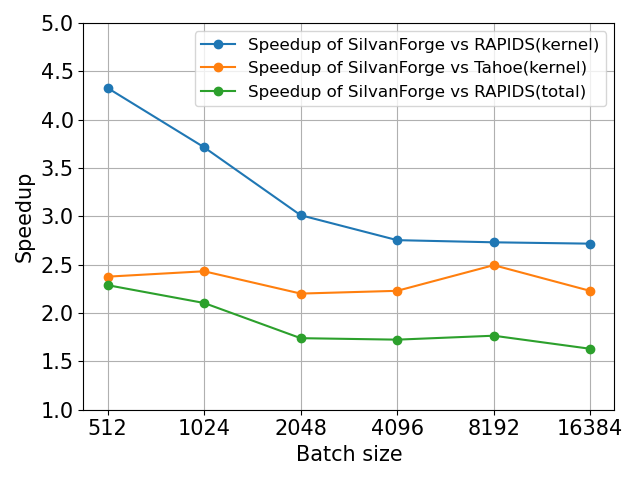
\includegraphics[width=\textwidth]{figures/geomean_speedup_4060_kernel_time_total_time.png}
      \caption{\label{Fig:TBvsRAPIDSTahoe_4060_Speedup}Speedup vs batch size}      
    \end{subfigure}
    \begin{subfigure}[t]{.32\linewidth}
      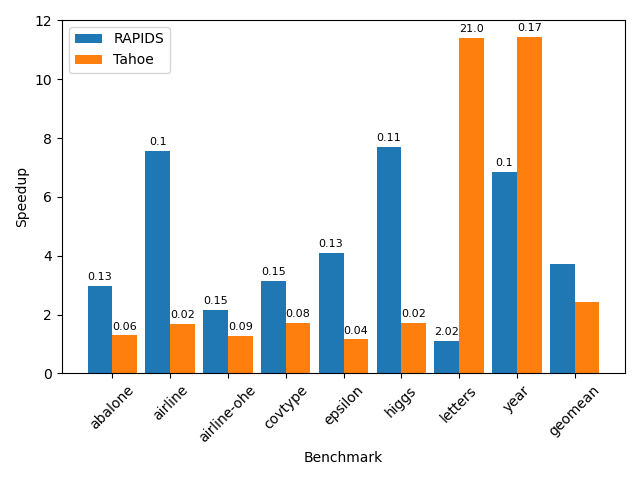
\includegraphics[width=\textwidth]{figures/speedup_bar_graph_1024.png}
      \caption{\label{Fig:KernelTimeIndividualBenchmarks4060a} Batch size 1024}
    \end{subfigure}
    \begin{subfigure}[t]{.32\linewidth}
      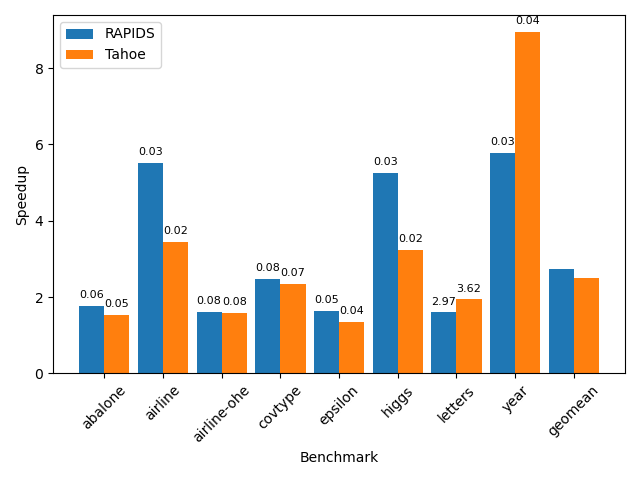
\includegraphics[width=\textwidth]{figures/speedup_bar_graph_8192.png}
      \caption{\label{Fig:KernelTimeIndividualBenchmarks4060b} Batch size 8192}
    \end{subfigure}
    % \hfill
    \caption{The first graph shows kernel and total time speedup of \Treebeard{} over RAPIDS and Tahoe (geomean over real-world 
    benchmarks) across batch sizes on NVIDIA RTX 4060. The bar graphs shows the kernel time speedup of \Treebeard{} per benchmark. Numbers on the bars are inference times per sample in $\mu$s for RAPIDS and Tahoe.}
\end{figure*}


% \begin{figure}[htb]
%   \centering
%   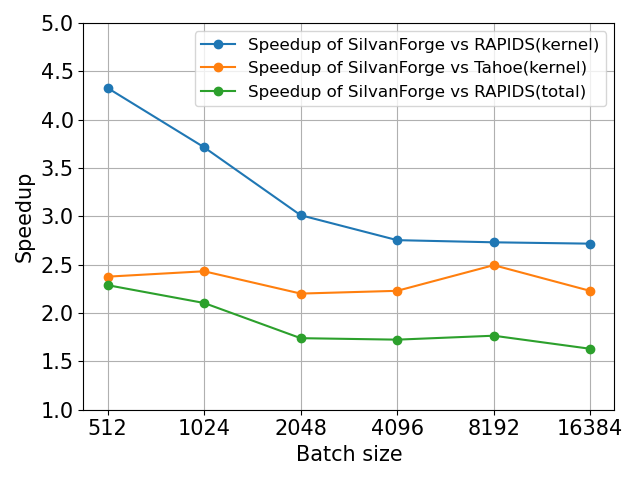
\includegraphics[width=0.75\linewidth]{figures/geomean_speedup_4060_kernel_time_total_time.png}
%   \caption{\Treebeard{} vs RAPIDS and Tahoe kernel time and total time speedup (geomean over real-world 
%   benchmarks) across batch sizes on NVIDIA RTX 4060}
%   \label{Fig:TBvsRAPIDSTahoe_4060_Speedup}
% \end{figure}

% \begin{figure}[htb]
%   \centering
%   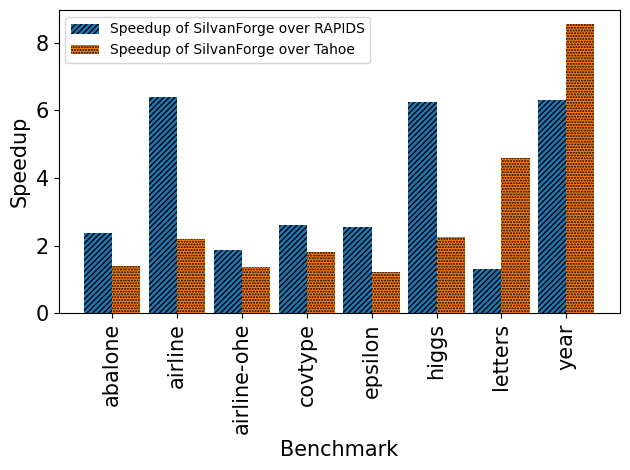
\includegraphics[width=0.75\linewidth]{figures/geomean_speedup_4060_bar_graph.png}
%   \caption{\Treebeard{} vs RAPIDS and Tahoe kernel time and total time speedup on NVIDIA RTX 4060 for individual benchmarks (geomean over all batch sizes).
%   \TODO{Add bar for total time. Add whiskers to each bar to show range of speedups.}}
%   \label{Fig:TBvsRAPIDSTahoe_4060_Speedup}
% \end{figure}

% \begin{figure*}[ht]
%   \centering
%   \begin{subfigure}[b]{.45\textwidth}
%     \subcaptionbox*{}{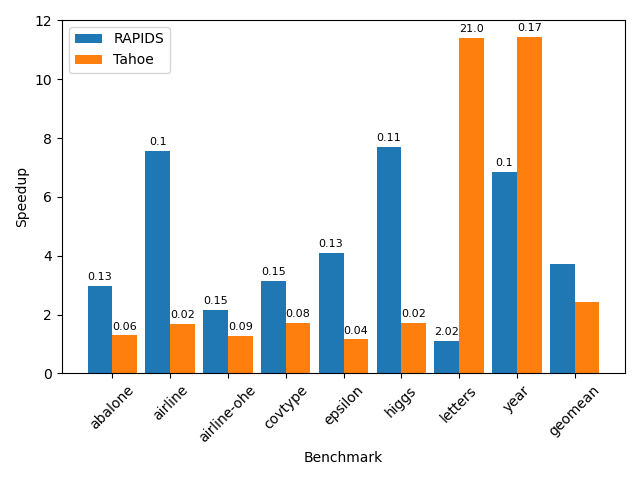
\includegraphics[width=\textwidth]{figures/speedup_bar_graph_1024.png}}
%     \caption{Batch size 1024}
%   \end{subfigure}
%   \begin{subfigure}[b]{.45\textwidth}
%     \subcaptionbox*{}{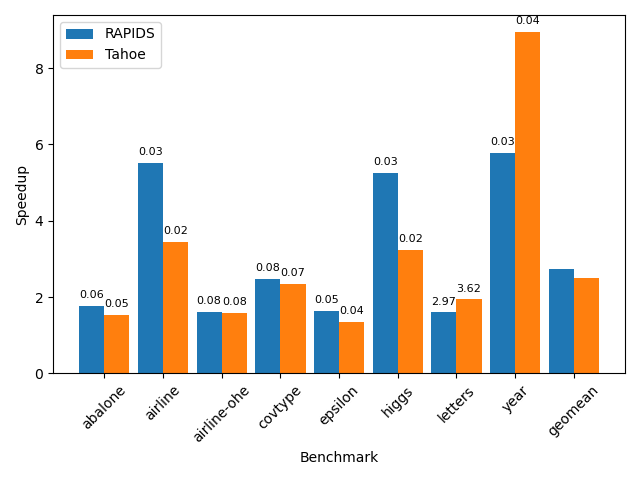
\includegraphics[width=\textwidth]{figures/speedup_bar_graph_8192.png}}
%     \caption{Batch size 8192}
%   \end{subfigure}
%   \hfill
%   \caption{\label{Fig:KernelTimeIndividualBenchmarks4060}Kernel time speedup of \Treebeard{} vs RAPIDS on NVIDIA RTX 4060. Numbers on the bars are 
%   inference times per sample in $\mu$s for RAPIDS and Tahoe.}
% \end{figure*}

Figures~\ref{Fig:KernelTimeIndividualBenchmarks4060a} and ~\ref{Fig:KernelTimeIndividualBenchmarks4060b} 
show per benchmark results at two different batch sizes. 
\Treebeard{} is able to find better schedules than both RAPIDS and Tahoe on each of the benchmarks. It consistently
outperforms both systems, achieving a speedup of upto $12\times$.
For about half the benchmarks, the speedup is $2\times$ or more over both baselines at batch size 8192.
% \begin{comment}
\subsubsection*{Synthetic models}
To establish that \Treebeard{} can consistently find betters schedules, we performed an exhaustive comparison between \Treebeard{} and RAPIDS on the 700 randomly generated models.   
Figure~\ref{fig:randomModels4060} the results at batch sizes 512 and 4096 on all models, on RTX 4060. 
Each plot shows the speedup of \Treebeard{} over RAPIDS along the z-axis, with the x-axis and y-axis representing the number of trees and the number of features. 
While the exact trends at different batch sizes vary it can be seen that \Treebeard{} consistently outperforms RAPIDS by $1.5-8\times$. Along the tree 
dimension we find that the speedup is very high with fewer trees and stabilizes at around $2\times$ from 300 onwards. We note that \Treebeard{} continues to scale well 
when the number of trees are increased even further. It achieves a speedup of around $2\times$ compared to RAPIDS on \op{letters}, a real-world benchmark
with 26K trees.

\begin{figure}[htb]
  \begin{subfigure}[t]{.475\linewidth}
    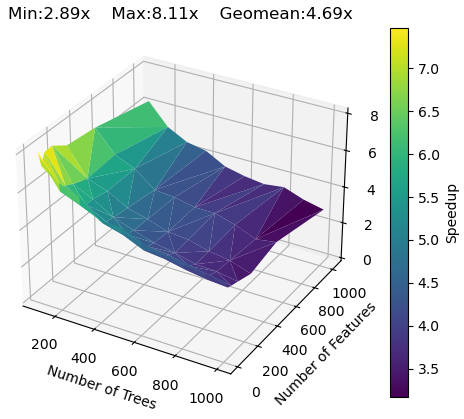
\includegraphics[width=\linewidth]{figures/RandomModels/kernel_speedup_b512_depth8.png}
    \caption{Batch size 512}
  \end{subfigure}
  \begin{subfigure}[t]{.475\linewidth}
    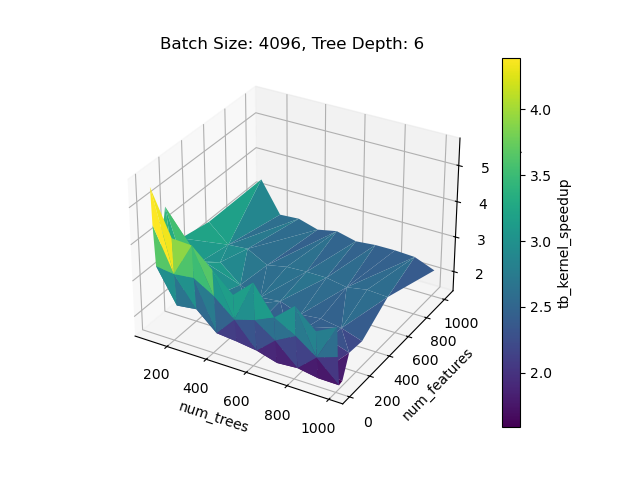
\includegraphics[width=\linewidth]{figures/RandomModels/kernel_speedup_b4096_depth6.png}
    \caption{Batch size 4096}
  \end{subfigure}
  \caption{\label{fig:randomModels4060}Kernel time speedup of \Treebeard{} over RAPIDS for random models.
  }
\end{figure}

\subsubsection*{Utility of Schedule Constructs}
A detailed analysis of the generated schedules indicate that caching, in-memory representation 
and reduction optimizations are crucial for performance. We observe that all three representations 
are necessary, array representation is used 60\% of the time, sparse 30\% of the time and reorg 
10\% of the time for the best schedules on the NVIDIA 4060.  
Next, shared reduction significantly improves performance especially for multi-class models. For example, 
the \op{letters} and \op{covtype} benchmarks achieve speedups of 1.5$\times$ with shared reduction (over the best schedule without shared reduction). 
Shared reduction increases the memory pressure (on shared memory) and not all schedules use it.
Finally, while GPUs have a hardware managed cache, explicitly caching the rows in shared memory using the scheduling primitives 
helps exploit the reuse of rows across trees. We find that caching rows is beneficial for many models
with speedups as large as $1.5\times$ over the best schedule without caching.

\subsubsection*{Comparison on T400}
To test the portability of \Treebeard{}'s techniques, we compare \Treebeard{} on the T400 GPU with RAPIDS and Tahoe. 
Figure \ref{Fig:TBvsRAPIDSTahoe_T400_Speedup} shows 
that even on the smaller GPU, \Treebeard{} is able to outperform them consistently (speedup always greater than $1.5\times$). 
As we adjust the batch size, we notice trends that are similar to those observed on the RTX 4060.

\subsection{Performance on AMD GPUs}
While Tahoe, RAPIDS and XGBoost only support NVIDIA GPUs, we demonstrate that \Treebeard{} 
is able to generate competitive code for AMD GPUs as well. \Treebeard{} can target AMD GPUs 
because it generates a combination of MLIR's \op{gpu} dialect and LLVM IR 
and these can be JIT'ed to AMD GPUs. While our objective here is not to compare directly 
between AMD and NVIDIA GPUs, we do find that the MI210 (which is more powerful) achieves better inference times 
on most benchmarks at large batch sizes ($\geq8$k). For example, at a batch size of 16k,
the MI210 is $2\times$ faster than the RTX 4060 on the \op{letters} benchmark. 

\subsection{Evaluation of the Schedule Exploration Heuristic}
We evaluated the schedule exploration heuristic described in Section \ref{sec:exploring} on several fronts.
Below we describe the major conclusions we can draw from the evaluation.

\subsubsection*{Efficacy and Speed of Scheduling Heuristic}
Figure \ref{Fig:HeuristicVsFullExplore_Speedup} compares the best schedule found by exhaustive exploration on the RTX 4060 
with the schedule found by the exploration heuristic.
The plot establishes that the 
heuristic is able to find schedules that are very close to the best schedule (well 
within 5\%). 
% The heuristic is consistently close to two orders of magnitude faster than exhaustive exploration. 
Importantly, the heuristic method is able to find good schedules in a fraction($1/80$-$1/100$) of the time taken by exhaustive exploration.
The exploration time ranges between $6$ and $167$ seconds for the heuristic with a mean of $28.7$ seconds.
These results show that our heuristic is able to quickly find schedules that are close to the best schedule.

\subsubsection*{Schedule Sensitivity Across GPUs}
We designed additional experiments to evaluate whether the best schedule (as picked by the heuristic) from one GPU can be used on another.
Figure \ref{Fig:AutotuningSpeedupvs4060Sched} reports the Geomean performance improvements of using the best schedule on T400 and MI210 compared to using the best schedule found on the RTX 4060 (for a given batch size).
As can be seen the T400 specific schedule is 1.05$\times$ to 1.2$\times$ better 
with the maximum difference being $2\times$ (\op{epsilon} at batch size 512).
There is a much larger variation in performance on MI120. For example, 
the geomean speedup over all benchmarks is 1.5$\times$ at batch size 16k (maxiumum 2$\times$ for the \op{letters} benchmark).
In conclusion, schedules found on one GPU do not carry over to other GPUs and often result in sub-optimal performance.
It is necessary tune schedules on each target to achieve the best performance.

\begin{figure*}[htb]
\begin{minipage}[t]{.3\linewidth}
  \centering
  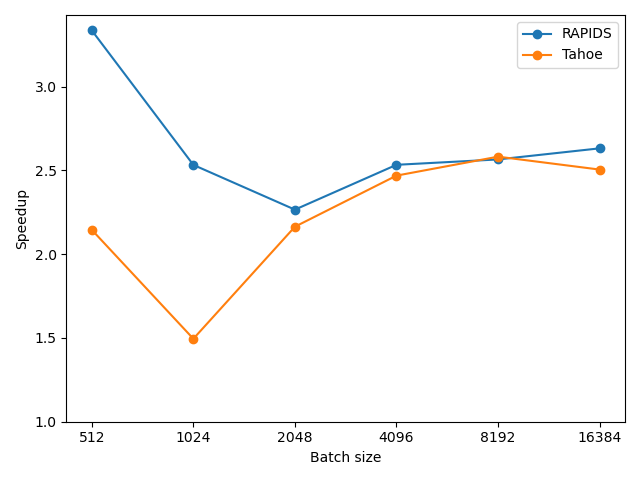
\includegraphics[width=\linewidth]{figures/geomean_speedup_T400_kernel_time.png}
  \caption{Speedup of \Treebeard{} over RAPIDS and Tahoe (geomean over real-world 
  benchmarks) across batch sizes on NVIDIA T400.}
  \label{Fig:TBvsRAPIDSTahoe_T400_Speedup}
\end{minipage}
\hspace{0.5cm}
\begin{minipage}[t]{.3\linewidth}
  \centering
  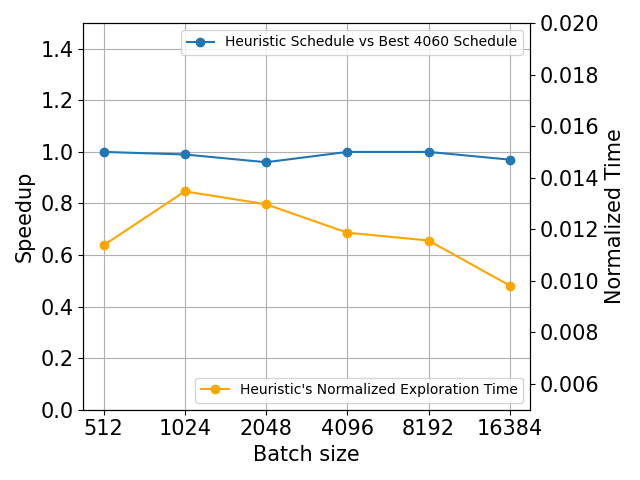
\includegraphics[width=\linewidth]{figures/speedup_vs_norm_time_line_graph_4060.png}
  \caption{Slowdown of heuristic schedule vs best schedule on NVIDIA RTX 4060 and 
  heuristic schedule exploration time normalized w.r.t full schedule exploration time.}
  \label{Fig:HeuristicVsFullExplore_Speedup}
\end{minipage}
\hspace{0.5cm}
\begin{minipage}[t]{.3\linewidth}
  \centering
  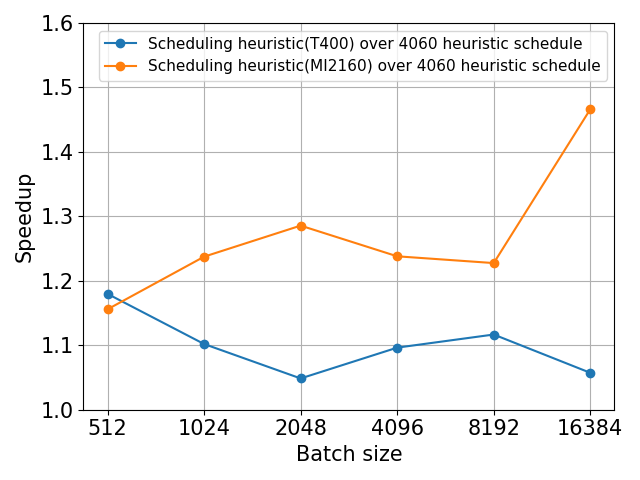
\includegraphics[width=\linewidth]{figures/geomean_speedup_T400_4060_vs_T400_vs_MI2160.png}
  \caption{Geomean speedup of using a hardware specific schedule on NVIDIA T400 and AMD MI210 over the best schedule from a different hardware (NVIDIA RTX 4060).}
  \label{Fig:AutotuningSpeedupvs4060Sched}
\end{minipage}
\end{figure*}

\subsection{CPU Improvements}
The enhancements made to the compiler enable \Treebeard{} to explore additional schedules on the CPU
compared to \TreebeardOLD{}. 
In particular, we find that the ability to parallelize across trees improves performance 
significantly at small batch sizes. At batch size 32, we find that the geomean speedup over 
all 8 real-world benchmark models is 2.2$\times$ with a max speedup of 5$\times$ (details omitted 
due to space constraints). At batch size 64, the average speedup
is 1.1$\times$ with a max speedup of 2$\times$. At batch size 32, parallelizing across trees is faster 
for all models and at batch size 64 the \TreebeardOLD{} schedule that parallelizes across 
rows is faster for only 2 of the 8 models. For small batch sizes, parallelizing across rows does 
not offer the best performance as there is limited reuse of trees in L1 cache.
Also, the amount of work per thread is very small leading to high overheads. 
Parallelizing across trees addresses both these problems. 

\subsection{Additional Observations}
%Beyond portable performance, our evaluation indicates that \Treebeard{} has several additional advantages over existing systems.
\subsubsection*{Cost Performance trade-off Across Hardware Platforms}
Two of the three GPU targets we use are commodity GPUs that cost less than \$400. They 
are infact much cheaper than the CPU we evaluate on. Despite this, performance on GPUs
is significantly better than on CPUs (by an order of magnitude on RTX 4060).
\Treebeard{} can therefore help data scientists make the best use of 
available processors on their systems.

\subsubsection*{A Note on batch size}
Batch size, exposes a trade-off between latency and throughput. It is not possible to use 
large batch sizes in latency sensitive applications. 
Ideally, one would like 
to maximize performance while respecting the batch size constraint imposed 
by the application. \Treebeard{} enables users to explore this trade-off.  
%\subsection*{}
\bigbreak
\noindent
Overall, our evaluation shows that \Treebeard{} is able to efficiently generate 
high-performance code for processors ranging from NVIDIA and AMD GPUs to Intel CPUs.
On all platforms and models that we tested on, \Treebeard{} significantly outperforms
state-of-the-art systems like RAPIDS, Tahoe, XGBoost and \TreebeardOLD{}.